\newpage
\section*{Appendix}\label{Appendix}
\appendix
\renewcommand{\thesubsection}{\Alph{subsection}}

%%%%%%%% DP Class %%%%%%%%%
\subsection{DP Class Requirements}\label{Sec:DP_Class_Requirements} 

\subsubsection{Equipment requirements}\label{Sec:Equipment_Requirements}
\begin{figure}[h]
    \centering
    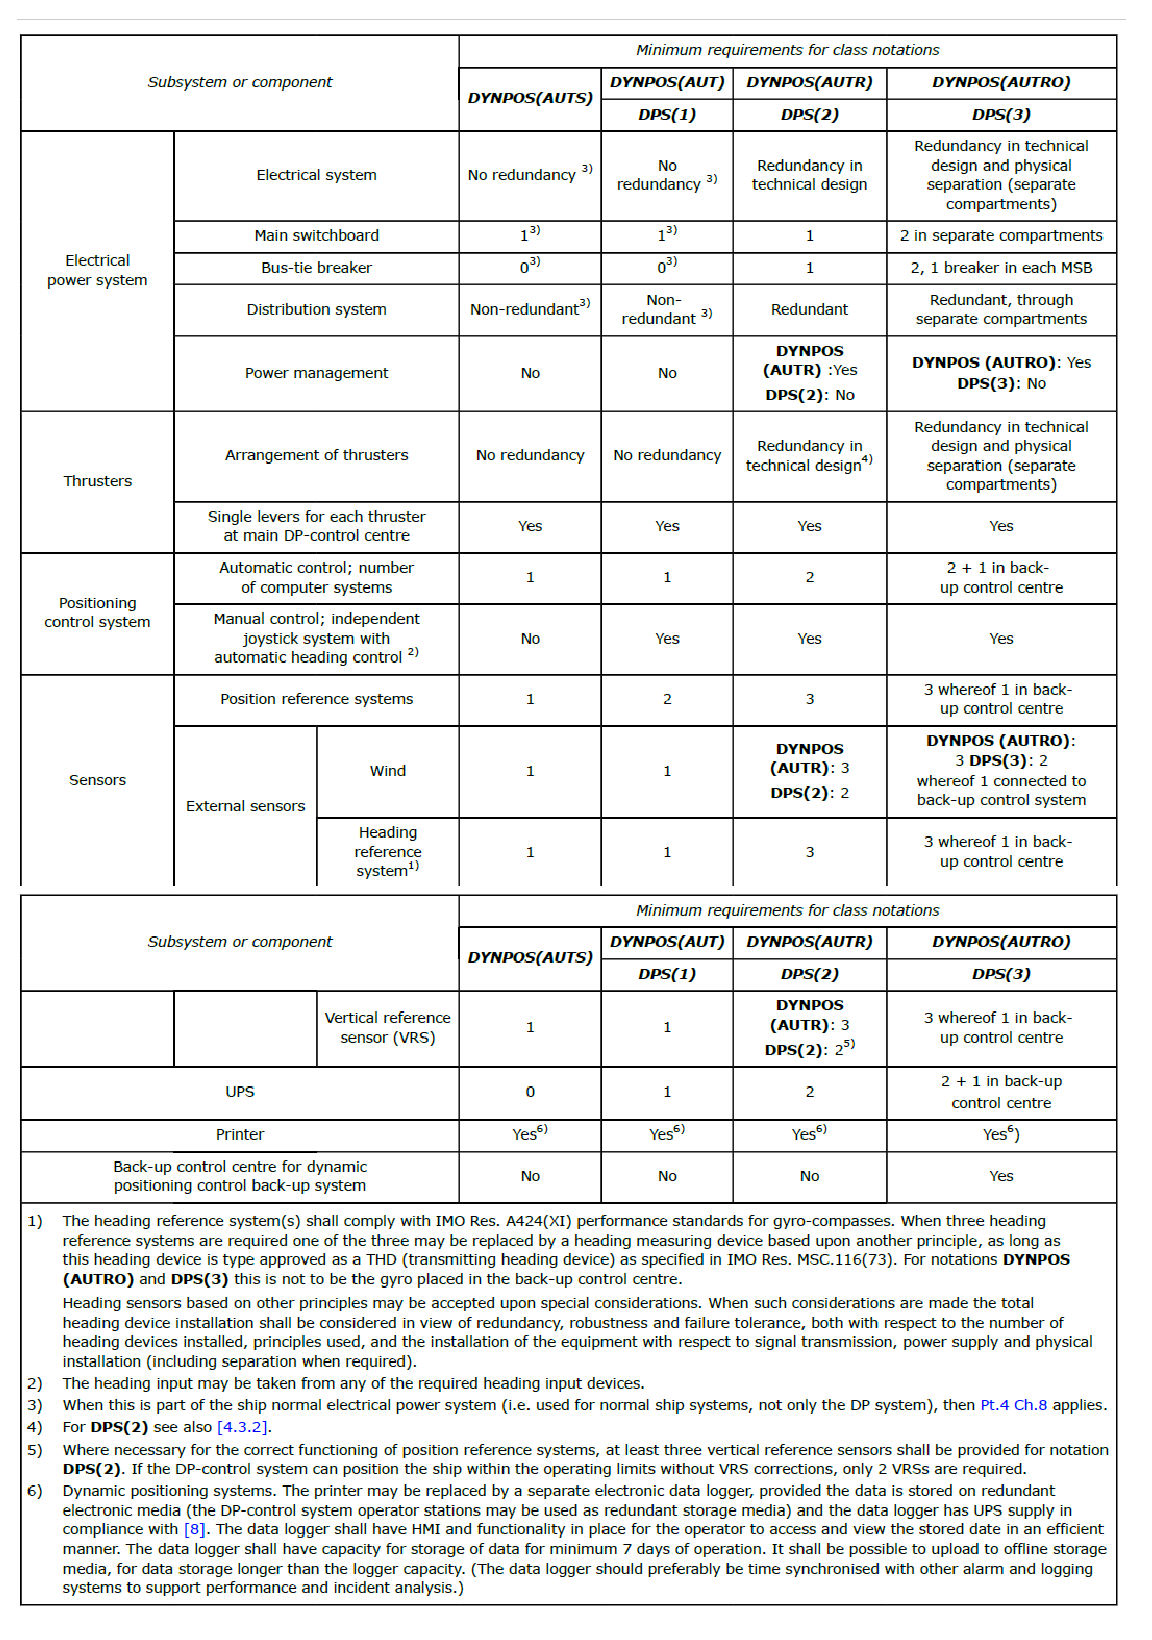
\includegraphics[width = 0.95\textwidth, height = 0.73\textheight]{figures/DP_requirements_table.eps}
    \captionof{table}{Minimum requirements for equipment on DP vessels for the different classifications \cite{DNV-GL_RP_Dynamic_positioning} .}
\end{figure}

\newpage
\subsubsection{Class Notations}\label{Sec:Class_Notations} 
\begin{figure}[h]
    \centering
    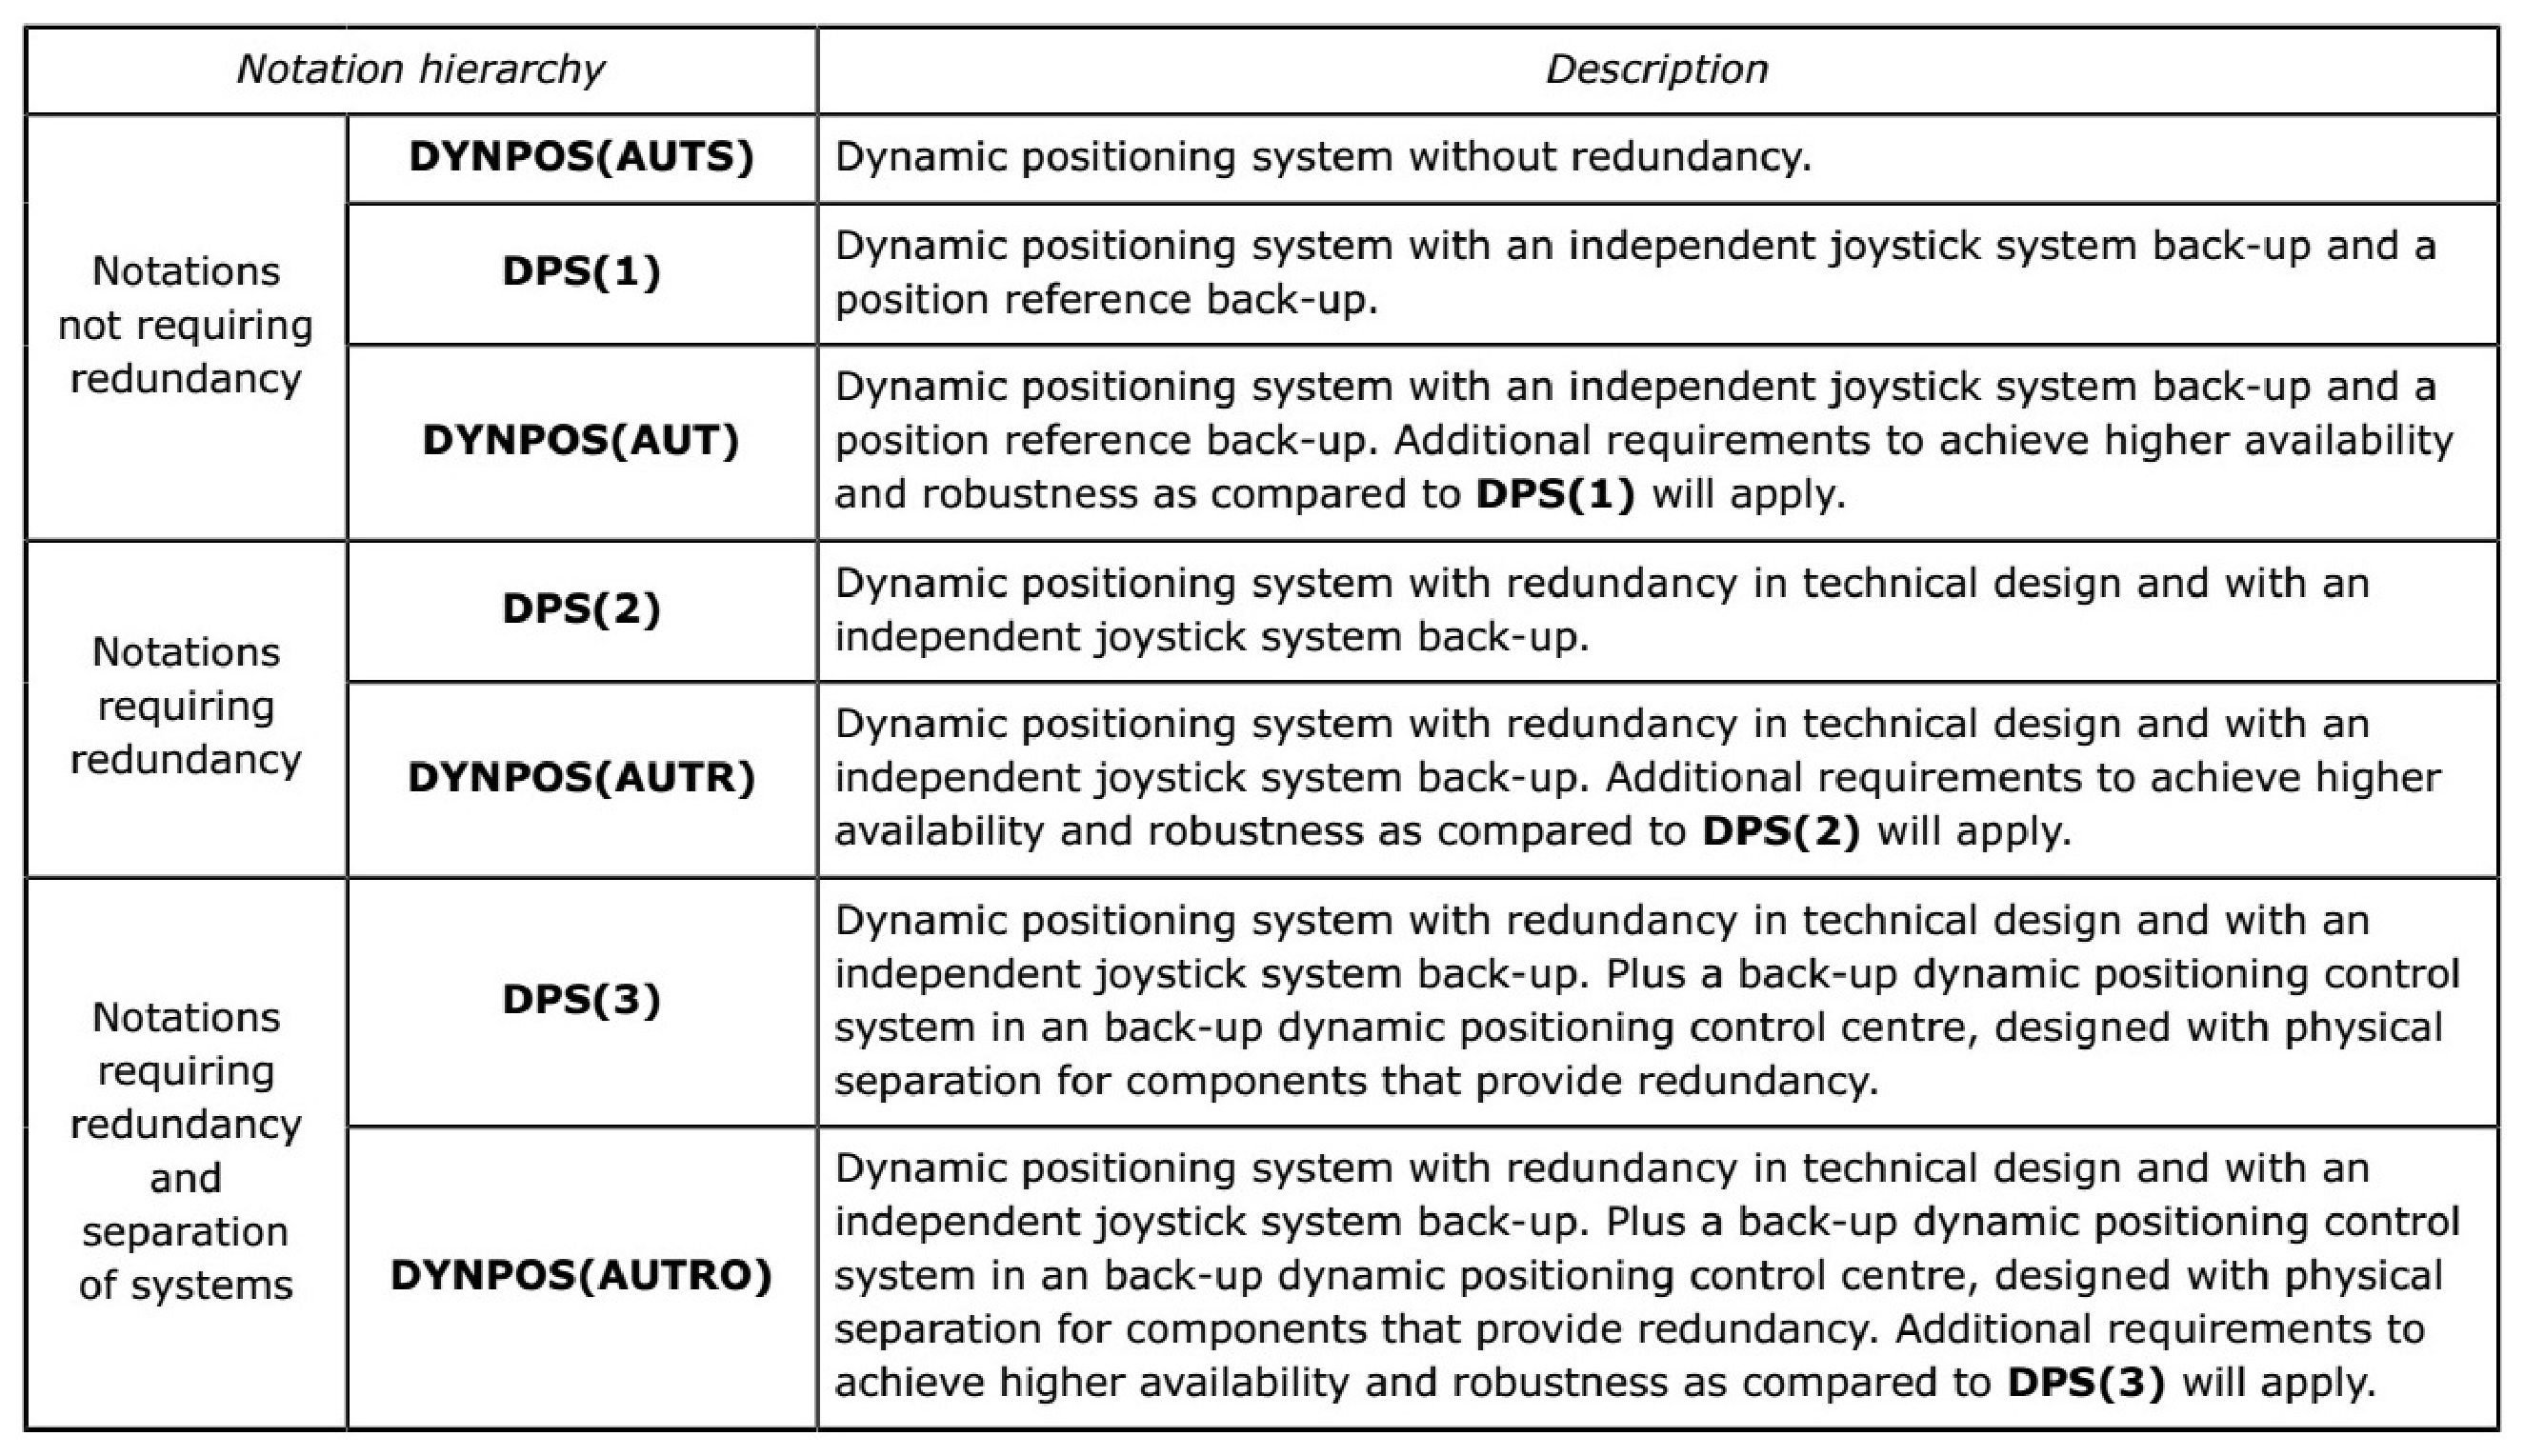
\includegraphics[width = \textwidth]{figures/DP_Class_notations.eps}
    \captionof{table}{Dynamic Positioning Class Notations. \cite{DNV-GL_Regulations_ship}}
\end{figure}

\subsubsection{DP Class Equivalent Notations}\label{Sec:Equivalent_Notations} 
\begin{figure}[h]
    \centering
    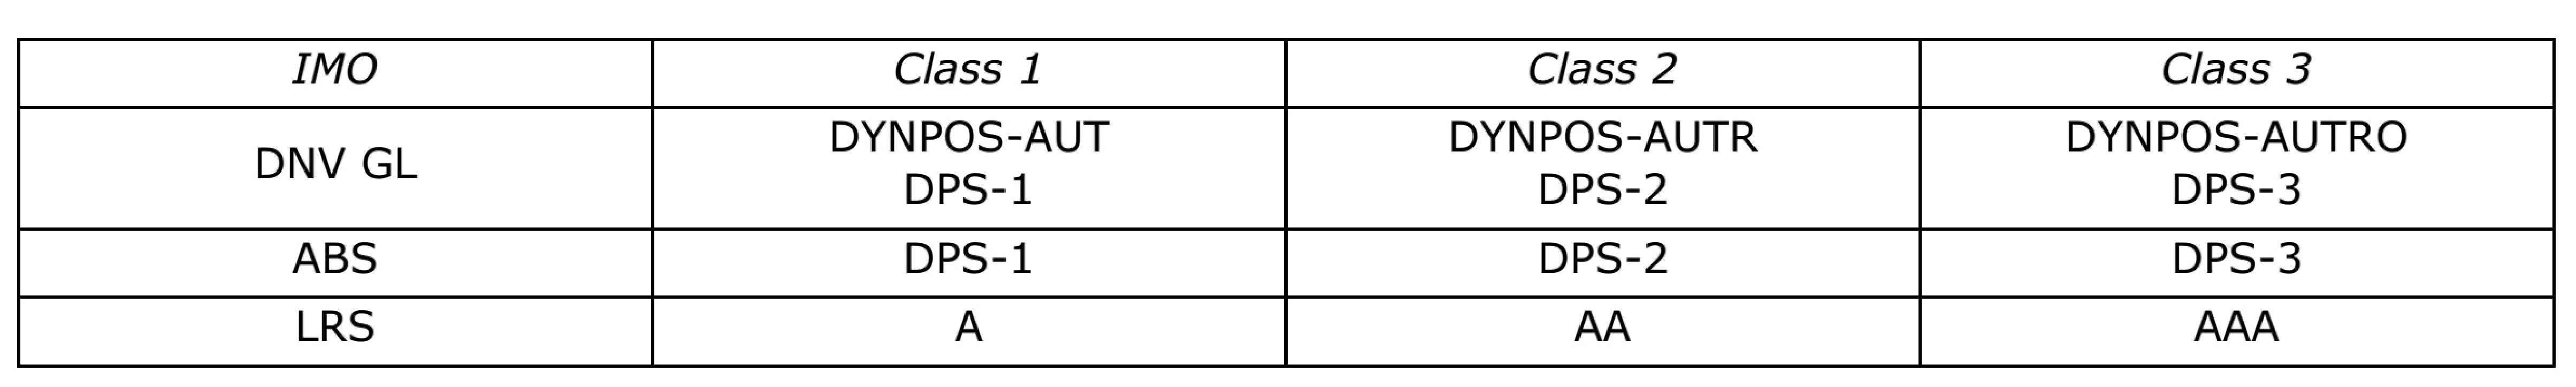
\includegraphics[width = \textwidth]{figures/DP_Class_equivalent_notations.eps}
    \captionof{table}{Class Equivalent Notations \cite[page.22]{DNV-GL_RP_Dynamic_positioning}}
\end{figure}


\newpage
\subsection{Single-line Diagrams}\label{Sec:Single-line_diagrams}
\begin{figure}[H]
    \centering
    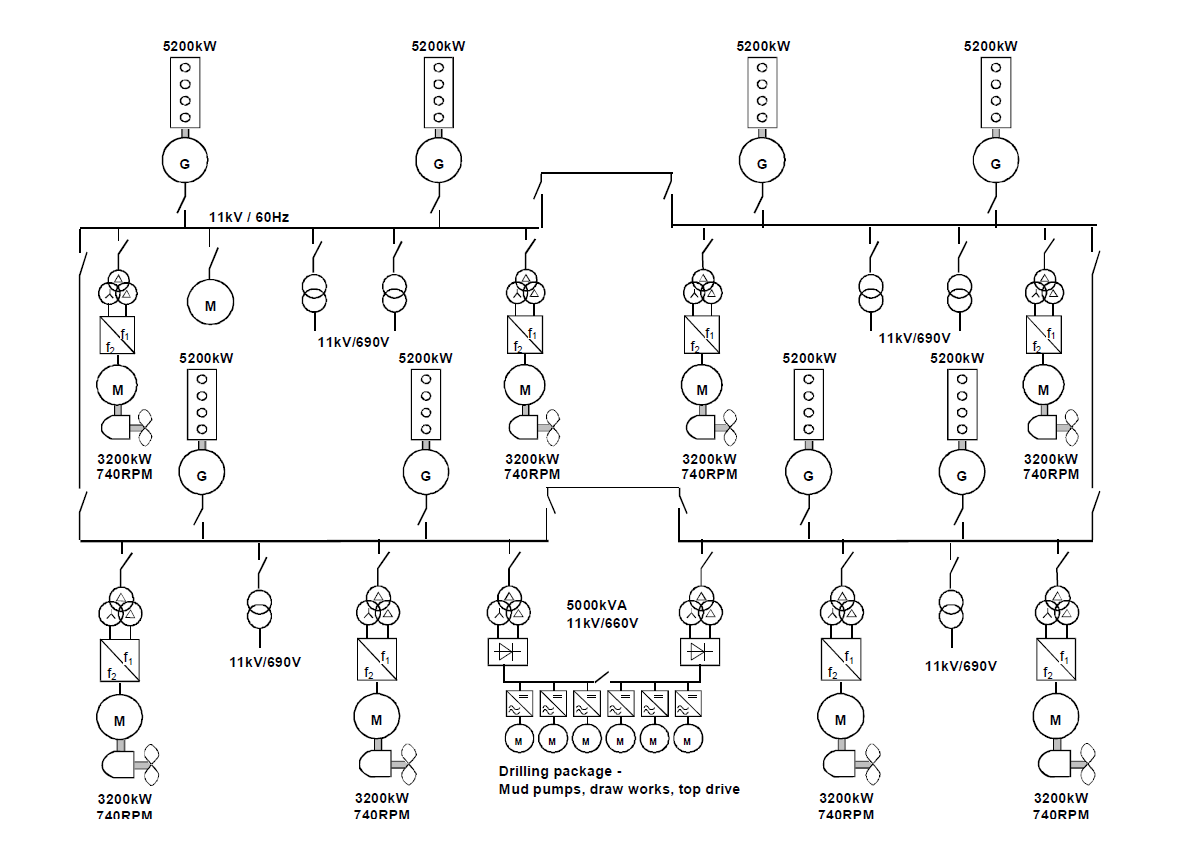
\includegraphics[width = \textwidth ]{figures/Comp_SingleLineDiagram.png}
    \caption{Single Line Diagram of a Semi-Sub \cite{MarReg1Comp}}
    \label{fig:Comp_SingleLineDiagram}
\end{figure}



\newpage
\subsection{Thruster Configurations} \label{Sec:ThrusterConfiguratons}
% \begin{figure}[h!]
%     \centering
%     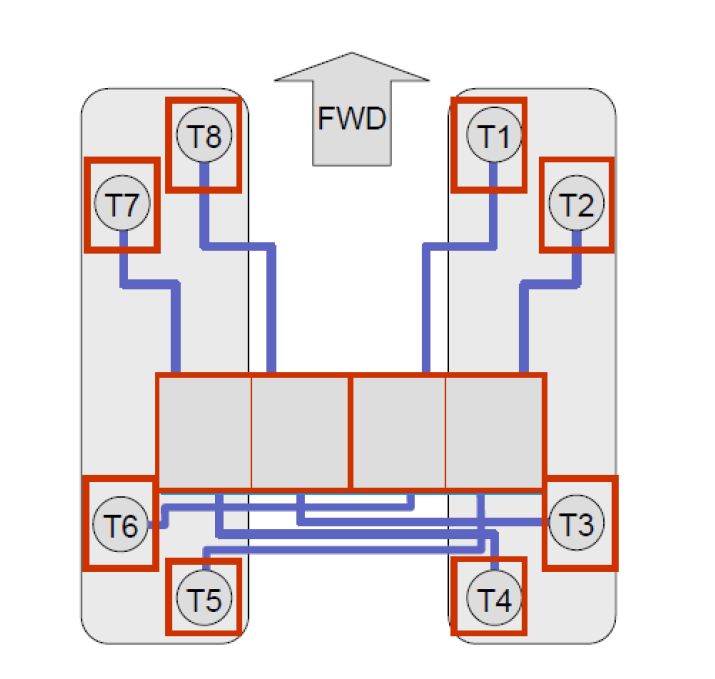
\includegraphics[width = \textwidth ]{figures/PP_RedundancyConfig.png}
%     \caption{Redundancy Configuration of a Semi-Sub \cite{LectureNote11PowerSystemDesign}}
%     \label{fig:PP_RedundancyConfig}
% \end{figure}

\begin{figure}[h!]
    \centering
    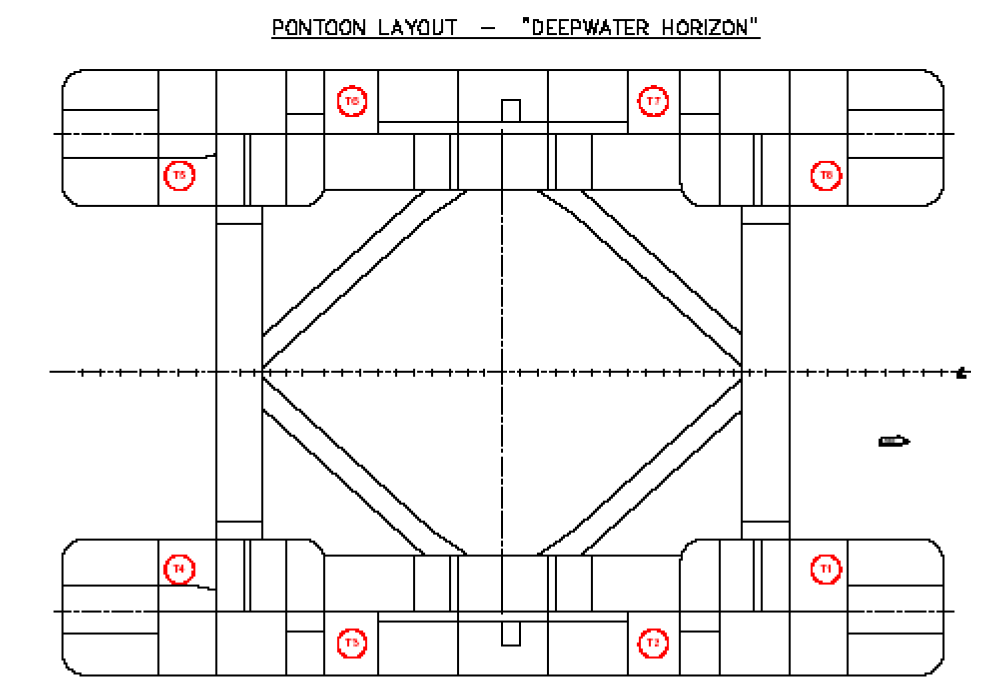
\includegraphics[width = \textwidth ]{figures/PP_ThrusterConfig.png}
    \caption{Thruster Configuration of the semi-sub "DEEPWATER HORIZON" \cite{LectureNote11PowerSystemDesign}}
    \label{fig:PP_ThrusterConfigDeepwaterHorizon}
\end{figure}

\begin{figure}
    \centering
    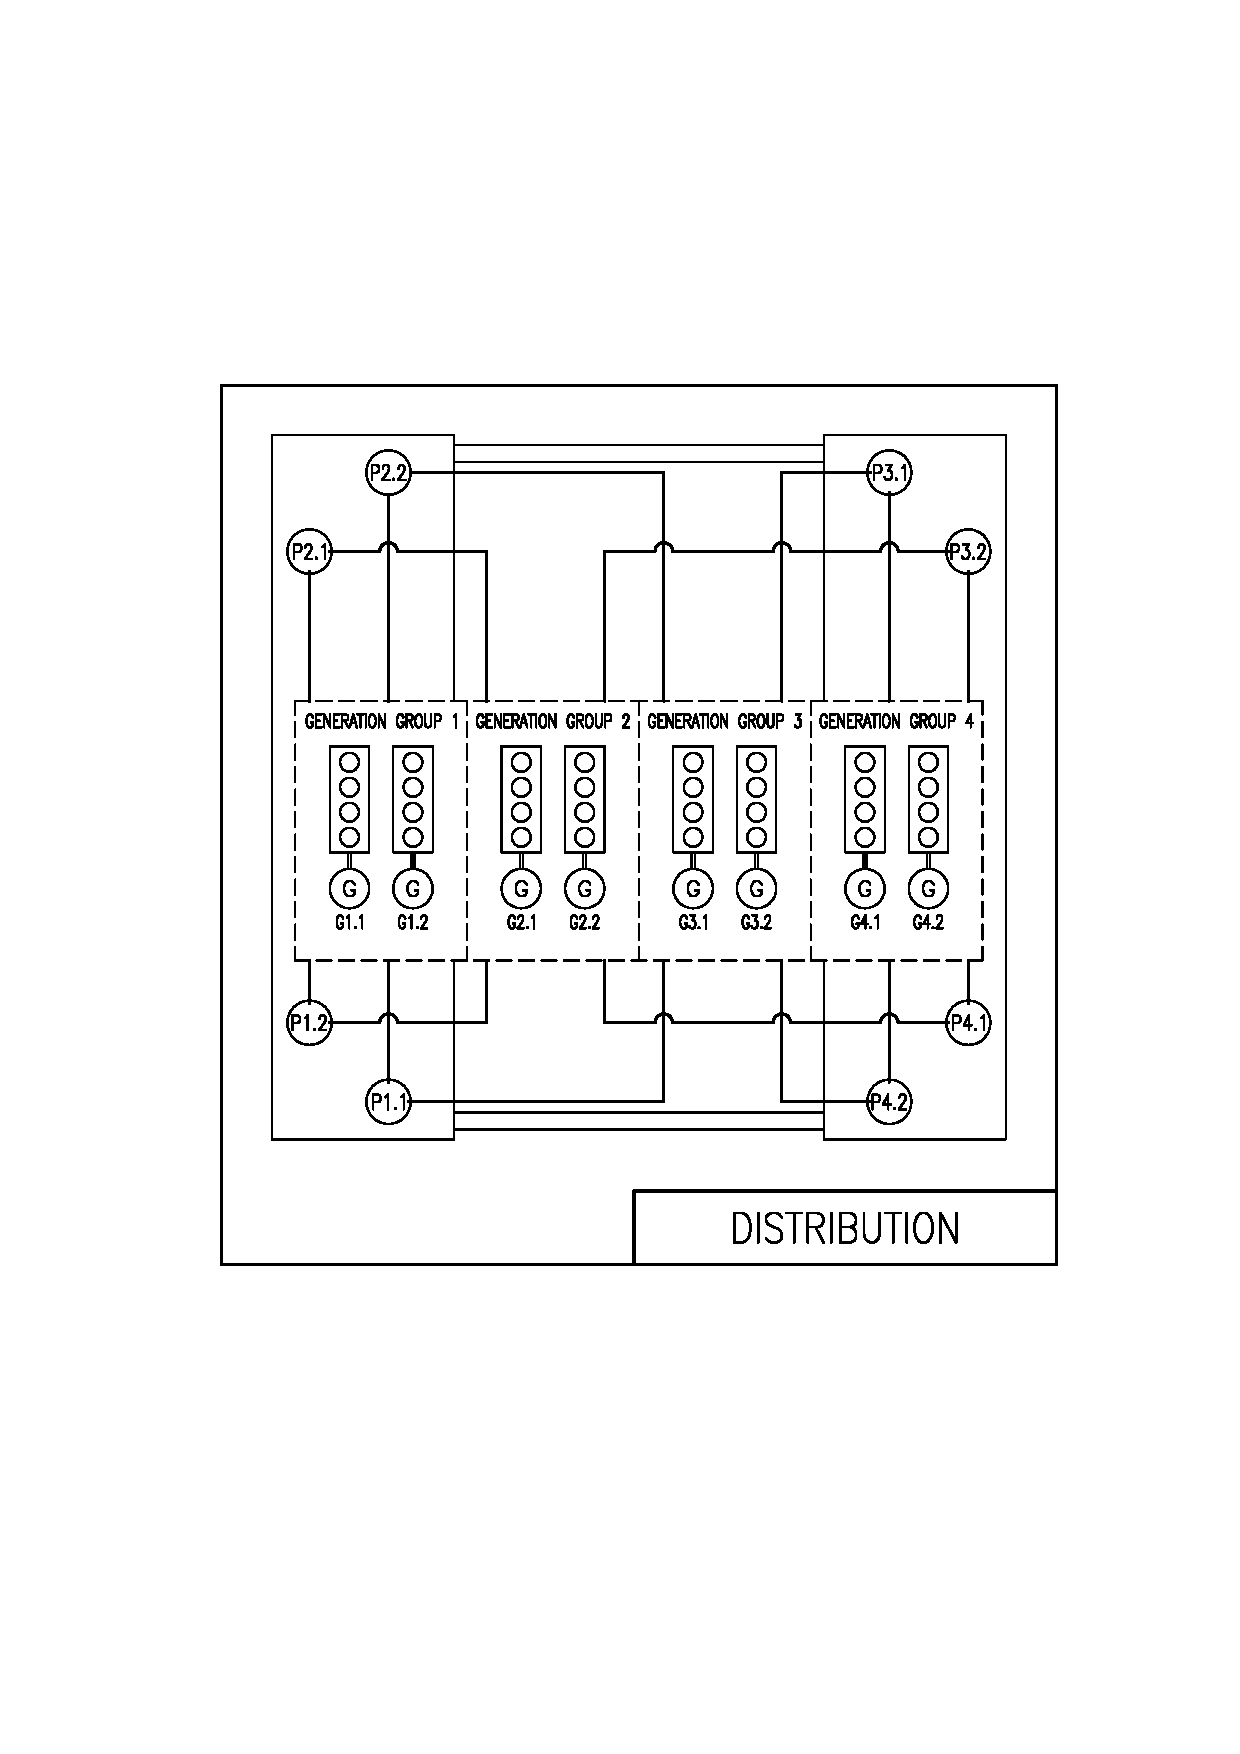
\includegraphics[width = \textwidth]{figures/Single_Line_distribution.pdf}
    \caption{Thruster configuration}
    \label{fig:SingleLineDistribution}
\end{figure}

\begin{figure}%[h!]
    \centering
    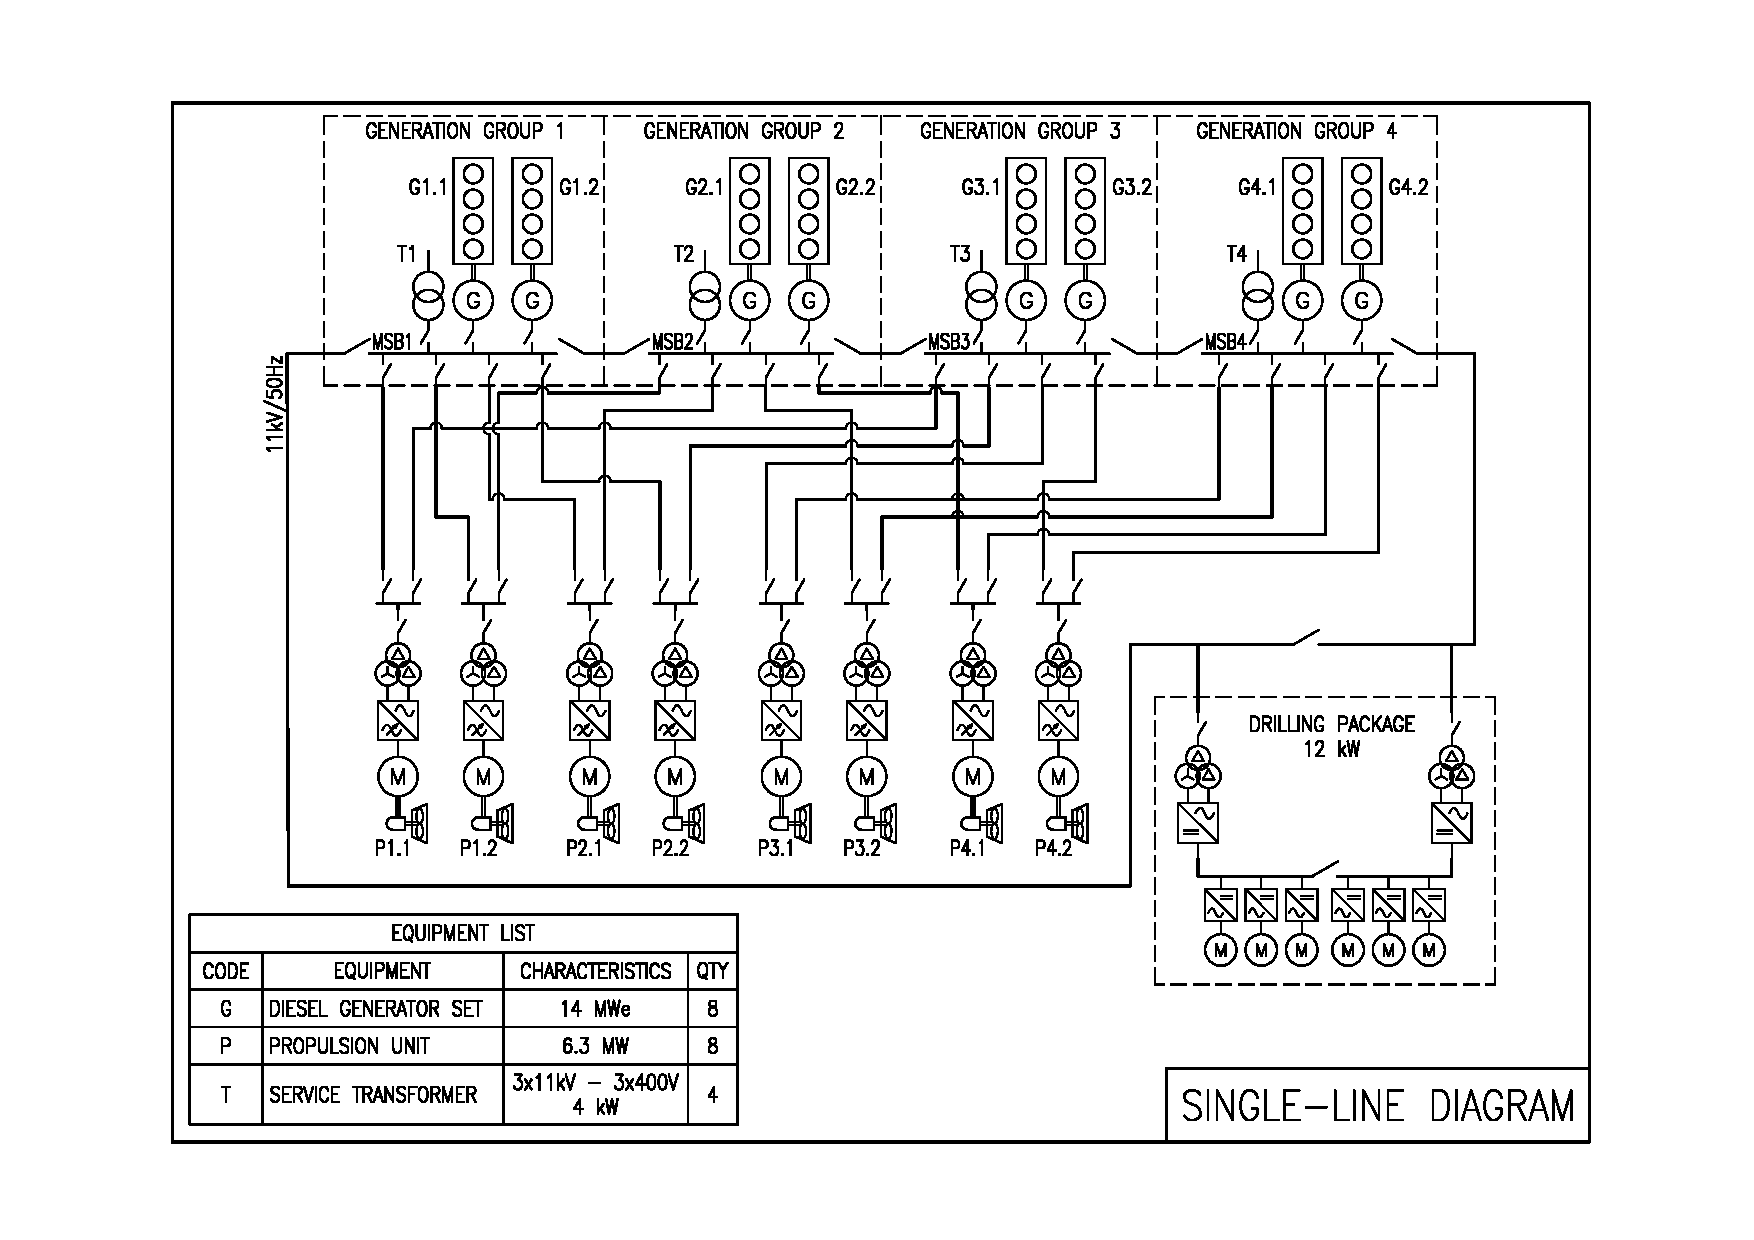
\includegraphics[scale=0.85, angle=90]{figures/Single_Line_diagram.pdf}
    \caption{Single line diagram}
    \label{fig:SingleLineDiagram}
\end{figure}

%The following comment with figure is only for making the single line figure appear. I don't know why Latex is not showing the last figure.
%\begin{comment}
\begin{figure}
    \centering
    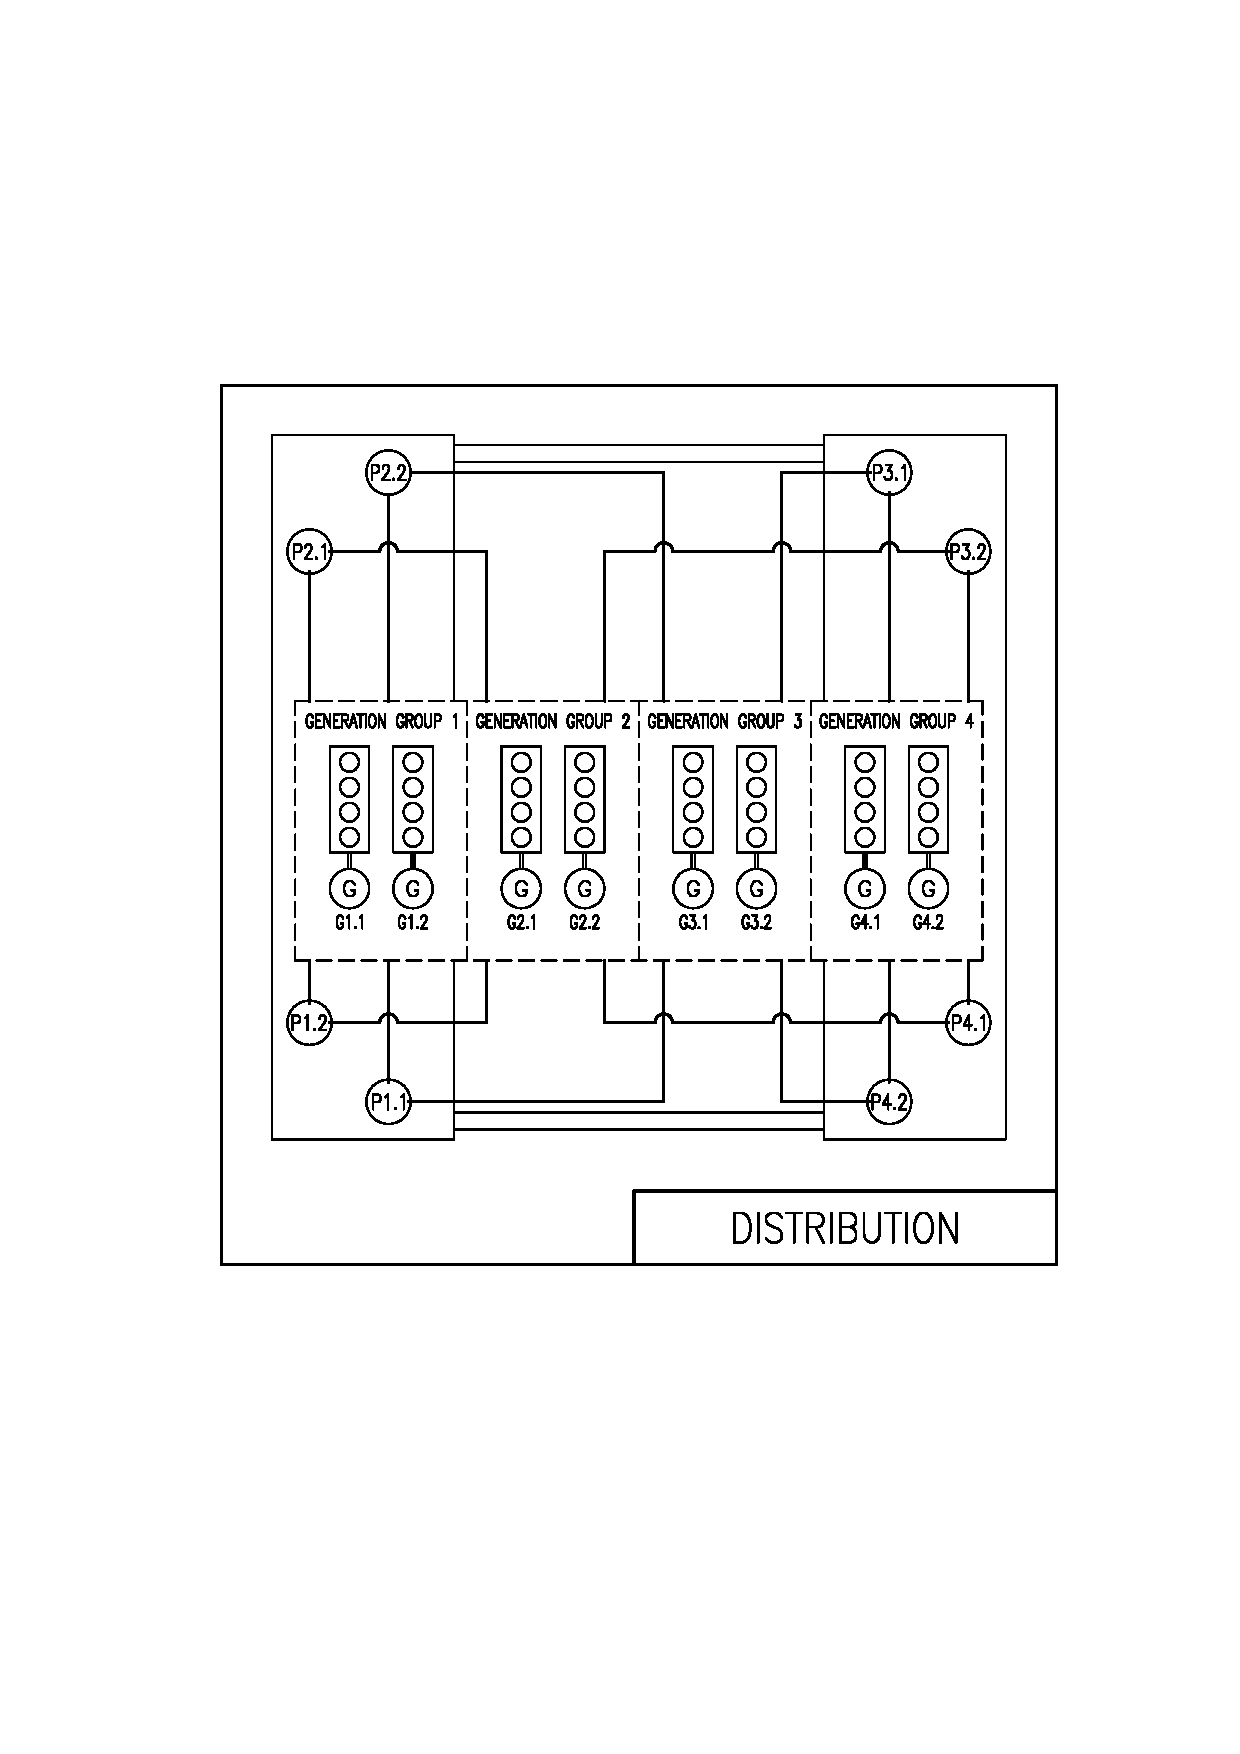
\includegraphics[width = \textwidth]{figures/Single_Line_distribution.pdf}
    \caption{Thruter configuration}
    \label{fig:SingleLineDiagram}
\end{figure}
%\end{comment}

% \subsection{Reference genset}\label{sec:referenceGenset}
% \begin{figure}
%     \centering
%     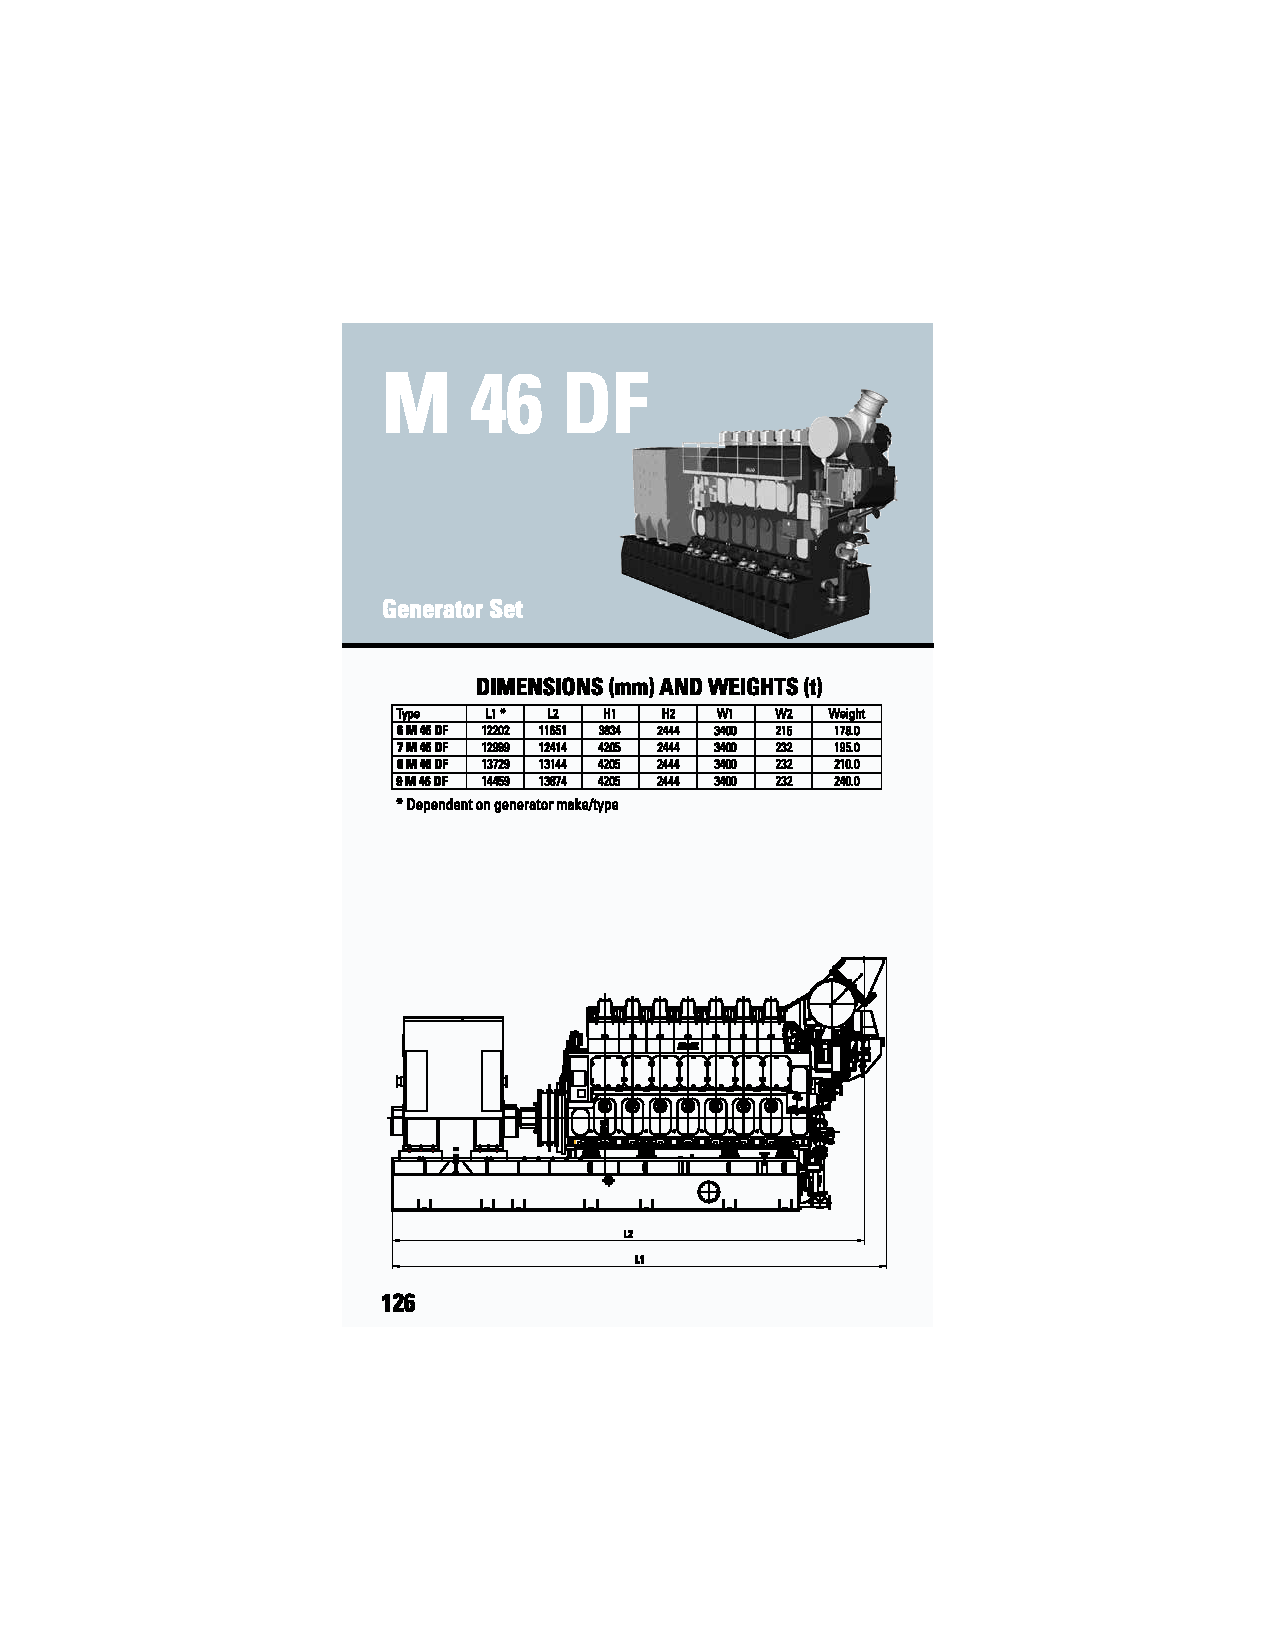
\includegraphics{figures/gensetDataWM46DF.pdf}
%     \caption{Date for the reference generator set WM46DF from Caterpillar Marine}
%     \label{fig:gensetDataWM46DF}
% \end{figure}